\documentclass[10pt, conference]{IEEEtran}

\usepackage{amsmath,amssymb,amsfonts}
\usepackage{algorithmic}
\usepackage{graphicx}
\usepackage{textcomp}
\usepackage{xcolor}
\usepackage{url}
\usepackage[backend=biber]{biblatex}
\addbibresource{mycite.bib}
\def\BibTeX{{\rm B\kern-.05em{\sc i\kern-.025em b}\kern-.08em
    T\kern-.1667em\lower.7ex\hbox{E}\kern-.125emX}}
\begin{document}

\title{Automatic Detection of Cryptographic API Misuses in Stack Overflow Java Code Snippets\\}

\author{\IEEEauthorblockN{Kristen Newbury}
\IEEEauthorblockA{University of Alberta \\
knewbury@ualberta.ca}
}

\maketitle

\begin{abstract}
Stack Overflow (SO) is a valuable platform for information for application developers. For this reason it is impertinent that the software development community considers the utility of code snippets distributed on the platform with a variety of metrics of software quality in mind. One crucial, but easily overlooked, metric of software quality is security. 

Recent work has applied manual classification to determine the security status of SO snippets. Other  work has applied machine learning to determine the security of code snippets on SO. There has also been work using static analysis on Android applications on Google Play that are considered to contain SO code snippets. No previous work has applied static analysis to accomplish automatically detecting insecure versions of Stack Overflow (SO) code snippets with respect to Cryptographic API usage.

In this study we aim to assess the viability of automating assessment of security directly on code snippets using a static analysis tool, CogniCrypt. We have extracted a sample of Java code snippets that use the cryptographic API, JCA, from SO and evaluated this sample of snippets to determine if there are misuses of cryptographic APIs present. We have found that 50\% of the total code snippets we were successful applying a relevant analysis to contained insecure usage of cryptographic APIs. 
\end{abstract}

\section{Introduction}
SO code snippets can be categorized as secure or insecure based on the viability of the code as a solution to security related task. Sometimes it is the case that a code snippet that objectively completes a task is insecure \cite{}. Insecurity in SO code snippets have a great implication. This is because it can be hard to concretely measure the cascading impact of an individual code snippet. 
Clearly posts with more views and answers that are accepted can be seen as sources of information with a higher likelihood of reaching many locations of use, but if  these end locations are proprietary, or if a snippet is pasted into code that is subsequently reused, it may be hard to trace eventually arising faults to the SO snippet.

Previous work \cite{} has looked at reasons that insecurity can arise in applications programming, specifically in terms of API usage. One insight of this study was that official API documentation can be lengthy and complex or non-present or insufficient as a resource for developers who are required to perform particular software development tasks. Another previous study \cite{} has found that SO has potential to be a valuable alternative source of information for developers. In a software development world where deadlines are real and efficiency of development processes are championed, SO is an attractive software development resource as it can enable developers to perform tasks quickly and efficiently. However, the same study also has found that it may not be the best source of information when it comes to performing security related application tasks.


A discussion of an ideal solution to assessing SO code snippet security is presented by these authors \cite{}. As they mention, an ideal solution would be to have a full automation of secureness classification. This ideal solution could be applied in two potential ways: as a check on the existing corpus of SO code snippets, with the possible goal of one of the following: alerting the author of the post to their presence, automatically tagging the post with a warning, or suggesting a fix. Another suggested outcome of such a work would be to integrated such a tool into the workflow of submission of posts to SO. The idea here is that the user submits a post, and in almost instant time the post is assessed for secureness and feedback is delivered if the post is insecure. Perhaps the submission is even rejected. In particular this second usage of such a pipeline tool could foster an awareness for good security practices in the software development community. While this work has not addressed either of these two goals directly, we believe that it would be viable to apply the work done here in either of these settings.

Recent work \cite{7958574} has used machine learning to classify security of code snippets traced from SO to Android applications on Google Play. 
 
 More recent work has focused on the security of code snippets on SO \cite{DBLP:journals/corr/abs-1901-01327}. 
 
 
Lastly we must acknowledge the inherently multifaceted nature of the notion of security. Security is complex, in that every layer of a system is affected by it, and even within layers there are multiple dimensions to the notion of security. One previous work \cite{} has observed that there are five main topics relating to security discussions in SO, some of these topics include web security, system security and cryptography. In this study we restrict our focus to application security, and specifically cryptographic security, via an evaluation of cryptographic API usage.

We classified security of code snippets concretely as either the presence or lack thereof cryptographic API misuses. We used the static analysis tool CogniCrypt \cite{krger_et_al:LIPIcs:2018:9215} to detect misuses. CogniCrypt is a static analysis tool that performs upon compiled Java bytecode that use cryptographic APIs and assess whether there exists some misuses of the API. Misuse is defined in a Domain Specific Language as a set of specifications over the entities that are relevant to that API. CogniCrypt is distributed with a ruleset for the Java Cryptography Architecture (JCA). The JCA is an architecture facilitating a standardized distribution of cryptographic task implementations.

In order to concretely investigate this area we have formulated the following research questions.


\begin{itemize}
\item  RQ1: Do cryptographic API misuses exist in code snippets from Stack Overflow?

\item  RQ2: What is the most common error detected in code snippets?

\item  RQ3: Can we estimate the impact of insecurity of code snippets>

\end{itemize}

\section{Tool Versions}

We strongly believe in the replicability of studies, as such we detail here the versions of tools used in our process such that any interested reader should be able to replicate as much of the setup of the study as possible.

The build of CogniCrypt that was used in this study roughly corresponds to release 2.0.0, but specifically was obtained from commit sha: 5f531d1d4377aefd35cec6658ae95308c6594244. The JCA ruleset was obtained as the zip download from release 2.0.0. 

Soot' partial program analysis (PPA) tool \cite{SootPPA} was used to perform compilation. One caveat of using this tool is that it is no longer maintained, and as such only provides full support of Java features for up to Java 1.4. We were required to make some source code changes to snippets to deal with such, as discussed below. These changes would not affect the semantics of the analysis that CogniCrypt performs.

\section{Dataset and Processing}



From this point we must define relevant code snippets for this study as code snippets containing Java code only, since CogniCrypt performs analysis upon Java bytecode. There is also the resulting requirement that the code snippets must be compilable. The previous studies that we have mentioned earlier that handle code snippet analysis of any sort have relied upon either AST or IR representation of the snippets, as the lowest level representation handled. They did not require the snippets to be compiled. This presents an additional complexity to our study. Code snippets, by definition, are partial programs. They often do not contain sufficient context to compile. Below we discuss in further detail the efforts necessary to deal with this, however these insights guide the rest of the data processing steps.

The dataset used for SO snippet collection this study was an sqlite import \cite{wong_2019} of the SOTorrent dataset released previously in an MSR submission \cite{}. In order to evaluate security of code snippets with CogniCrypt we collected snippets related to both security and java. 

In gathering data we performed the following steps in order to gather a relevant and reasonable set of code snippets to evaluate.

\subsection{Identifying Answer Posts Containing Java Security Snippets}
In the process of identifying java code snippets, only snippets from answer posts were considered. This was because of the intuition that answer posts are more likely to be a source for code that will be copied into a project, as noted in previous work \cite{7958574}. Code snippets were identified as Java Security related if they originated from answers to posts that were labelled with the both the “java” and "security" tag on Stack Overflow. Posts annotated with java-ee and java-se were not explicitly sought out, from the intuition that posts with these tags mostly also had the java tag as well. As well, only accepted answers posts were considered, as it can be argued that the answer that will be utilized the most will be the accepted answer, and that often the rest of the answers are less utilized. Only the latest version of a post was examined, as this is assumed to fairly represent what an author intended to share at that time. Analysing previous versions of a post would not be fair because bug fix edits may have been made to a post at some point in time, and separately modelling all versions of posts would not realistically give us an indication of overall security at one point in time. Finally, each code block of a post is treated as a separate snippet.  


\subsection{Identifying Crypto Security Related Posts}
In order to collect usages of crypto APIs specifically, considering that CogniCrypt uses a ruleset tailored to the JCA, we also filtered our dataset for snippets using a particular set of keywords. 
Normally a reasonable process to identify API usage of a piece of java software would be to look at the import statements listed in the project, however because of the partial nature of code snippets this technique would not work. We found that only approximately 6\% of the code snippets of our sample contained at least one import. It is likely that SO authors assume that the user of the code snippet can obtain the resolution of Objects themselves, and that they will supply the missing import statement.
In order to then identify usages of cryptographic libraries we only retained code snippets that contained at least one of the following keywords:

\begin{itemize}
  \item Provider
  \item Security
  \item SecureRandom
  \item MessageDigest
  \item Signature
  \item Cipher
  \item KeyFactory
  \item KeyGenerator
  \item KeyAgreement
  \item KeyStore
  \item CertificateFactory
  \item KeyPair
  \item KeySpec
  \item AlgorithmParameter
\end{itemize}

 
These keywords were chosen as they are listed by in the JCA documentation \cite{JCA} as the core classes and interfaces of the JCA.

One issue here that we considered is that the names of methods and objects in a partial program are only identified by partially quantified names (PQN). A complete program will have full quantified names (FQN) for objects at the compilation step. The problem here is that there logically cannot be a constraint on Java as a programming language that would prevent multiple classes from different packages from having the same name, and in fact that is completely unnecessary, as a FQN is unique. The problem only arises when we are not provided information about the provider of a class (recall that only 6\% of the snippets had an import). One example of this can be seen in java.util.Date and java.sql.Date. Both classnames are Date, however they are clearly provided by different packages and should be handled as unique.

Previous works \cite{} have investigated resolving PQN to FQN by using variants of oracles to determine which possible types the ambiguous class name or method name could actually resolve to. In many cases, given a concrete implementation of a standard library, it is easy to tell if a class name corresponds to a valid type in that library. 

When it is the case that there could be multiple resolutions, it would be semantically incorrect to treat the object as any of those. This is highly relevant in our study since CogniCrypt's ruleset is defined over specific types, and an attempt to apply those rules to a "similarly" named but semantically inequivalent implementation would ruin the foundations of the analysis.

Luckily Soot PPA handles this for us,in a way it is our oracle. It works to perform type recovery when it can, and in the case that a type is ambiguous and cannot be recovered, it makes a safe approximation of that object by classifying it as unknown. This is completely safe, as then the object is still modelled loosely in the bytecode representation of the snippet, but CogniCrypt obviously does not have any rules for unknown objects and therefore will not report them as the source of violations of rules.

\subsection{Compilation of Snippets Using Soot PPA}

As previously mentioned we had to deal with the constraint that the snippets needed to be compiled.

After assessing which snippets could not be successfully compiled, we were left with a sample of to run CogniCrypt on. 

\section{Results}

\subsection{RQ1}

We discovered that we were indeed able to analyze some of the snippets. 
\begin{figure}[h]
\begin{center}
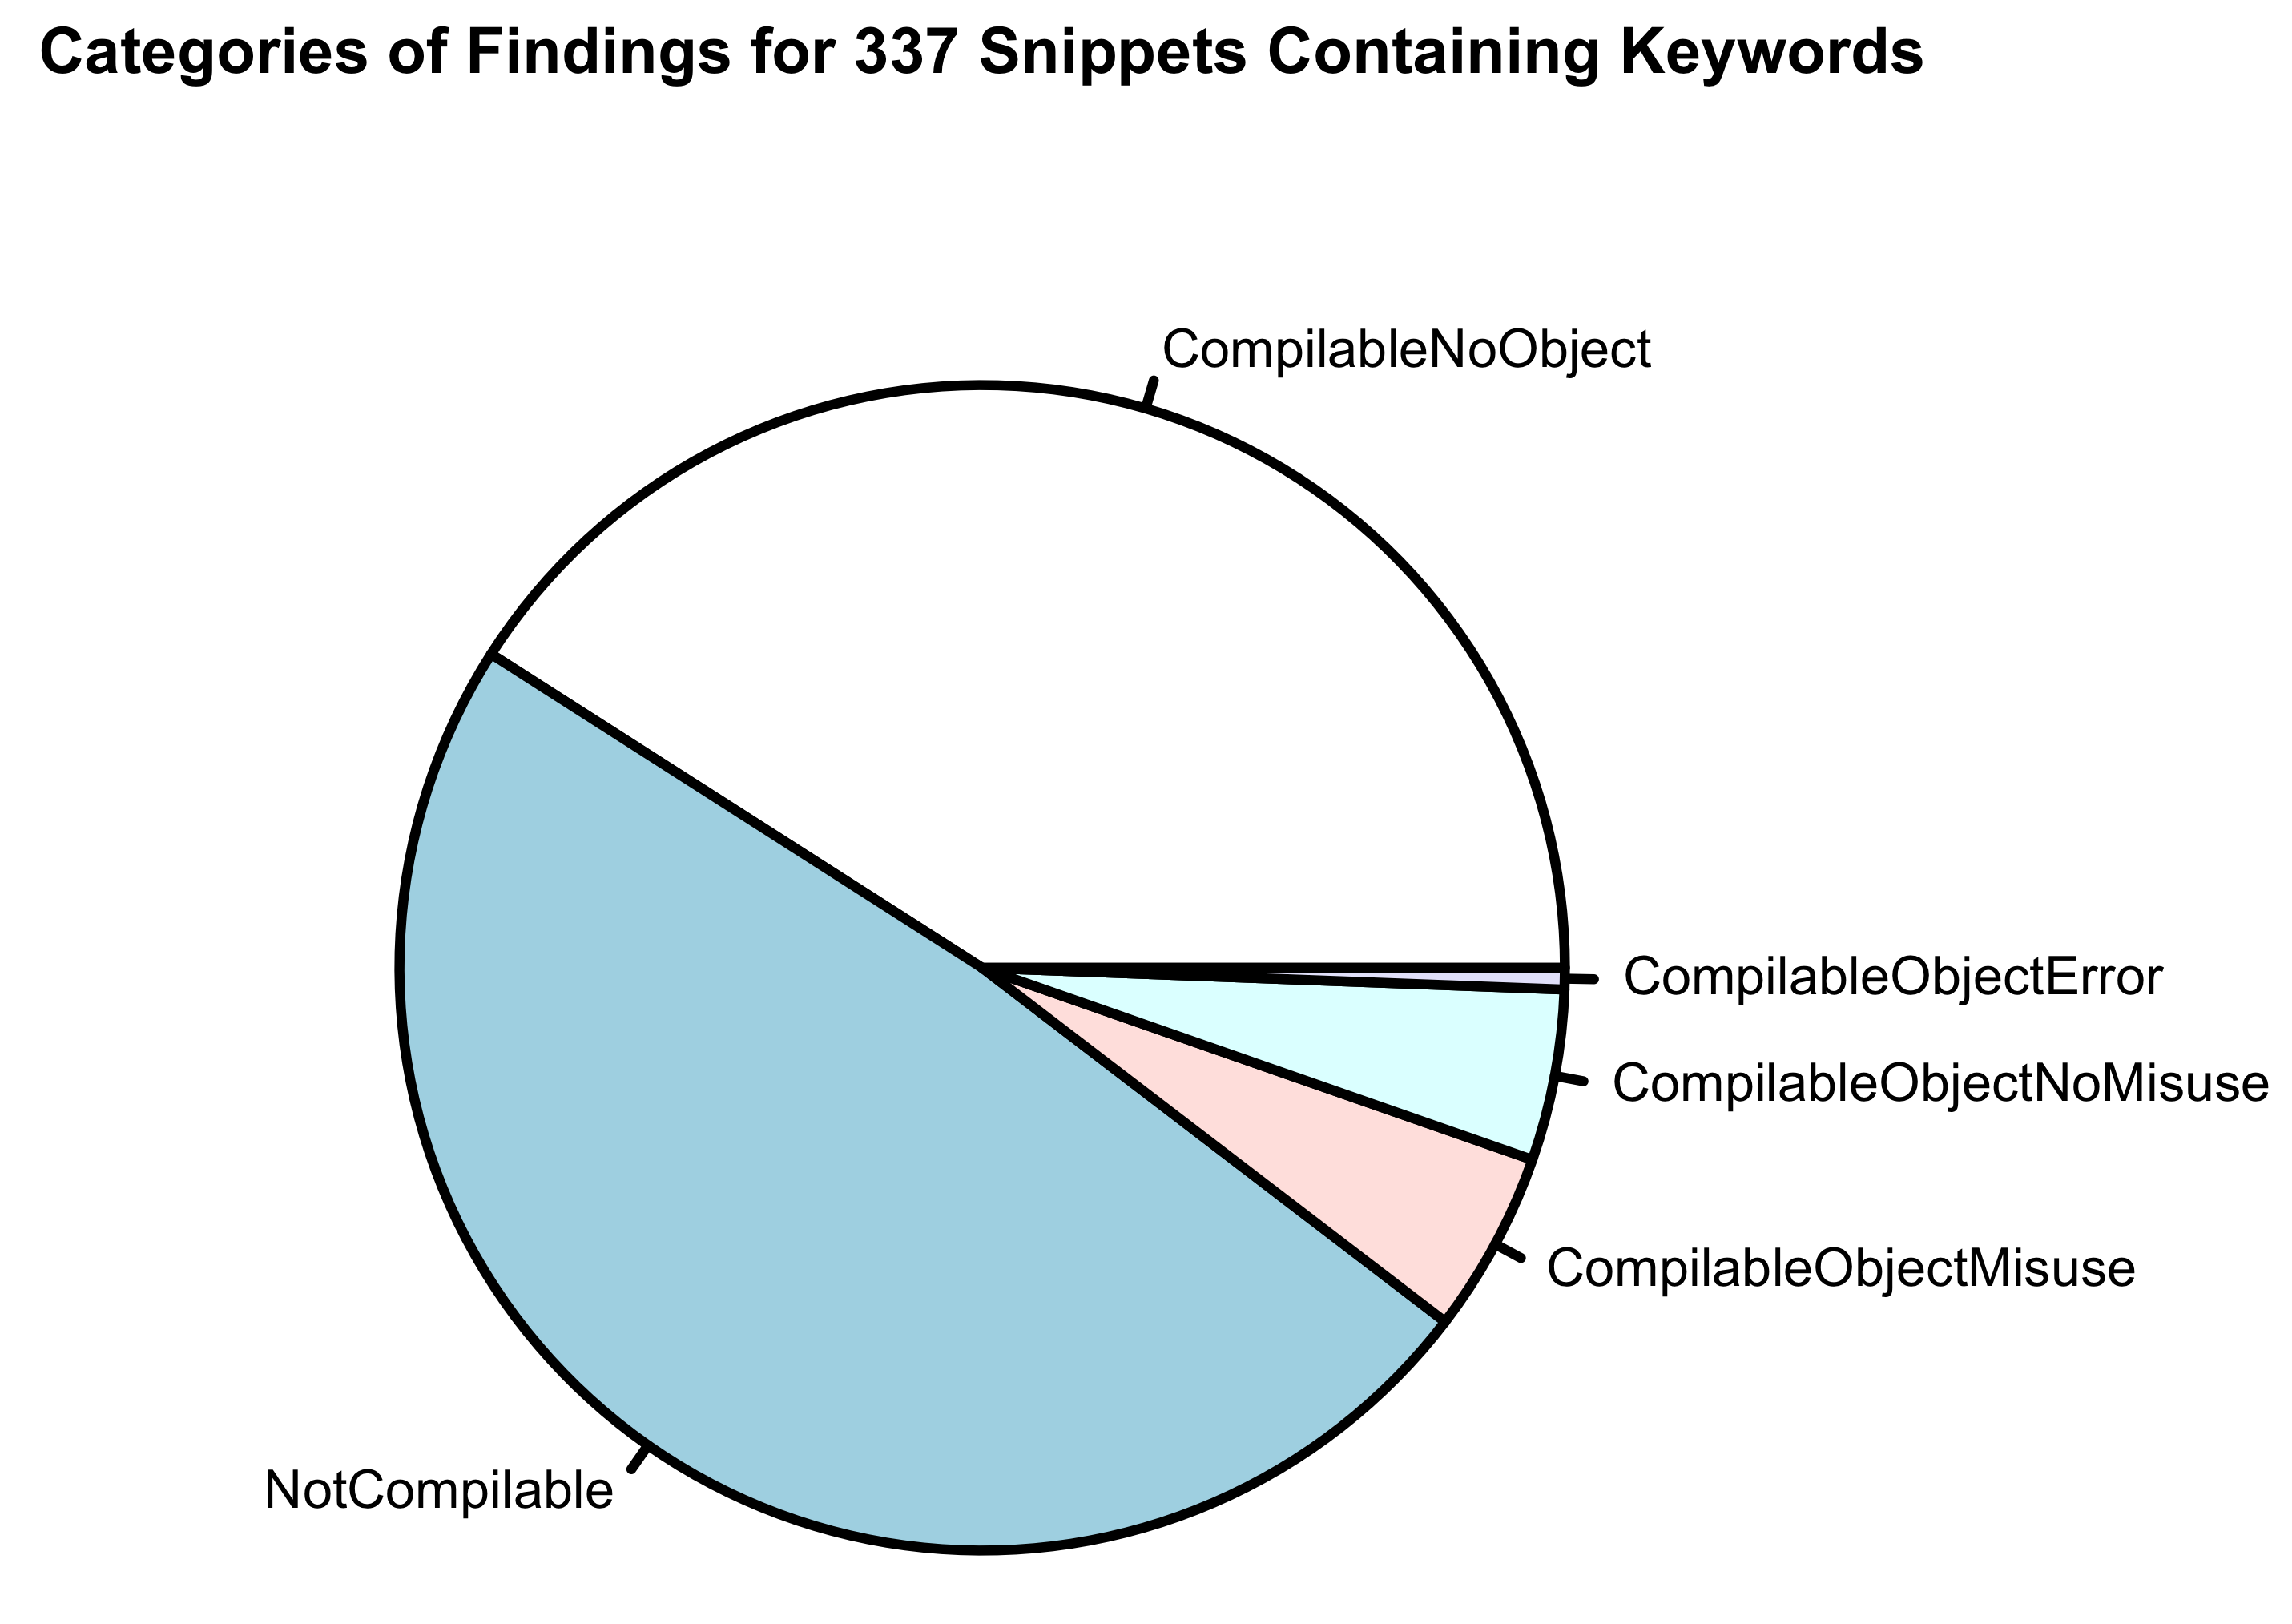
\includegraphics[width=.75\linewidth]{Pie.png}
\caption{Counts of Snippets at Each Level of Processing}
\end{center}
\end{figure}

\subsection{RQ2}

The distribution of errors as reported by CogniCrypt is presented in Fig 2.

\begin{figure}[h]
\begin{center}
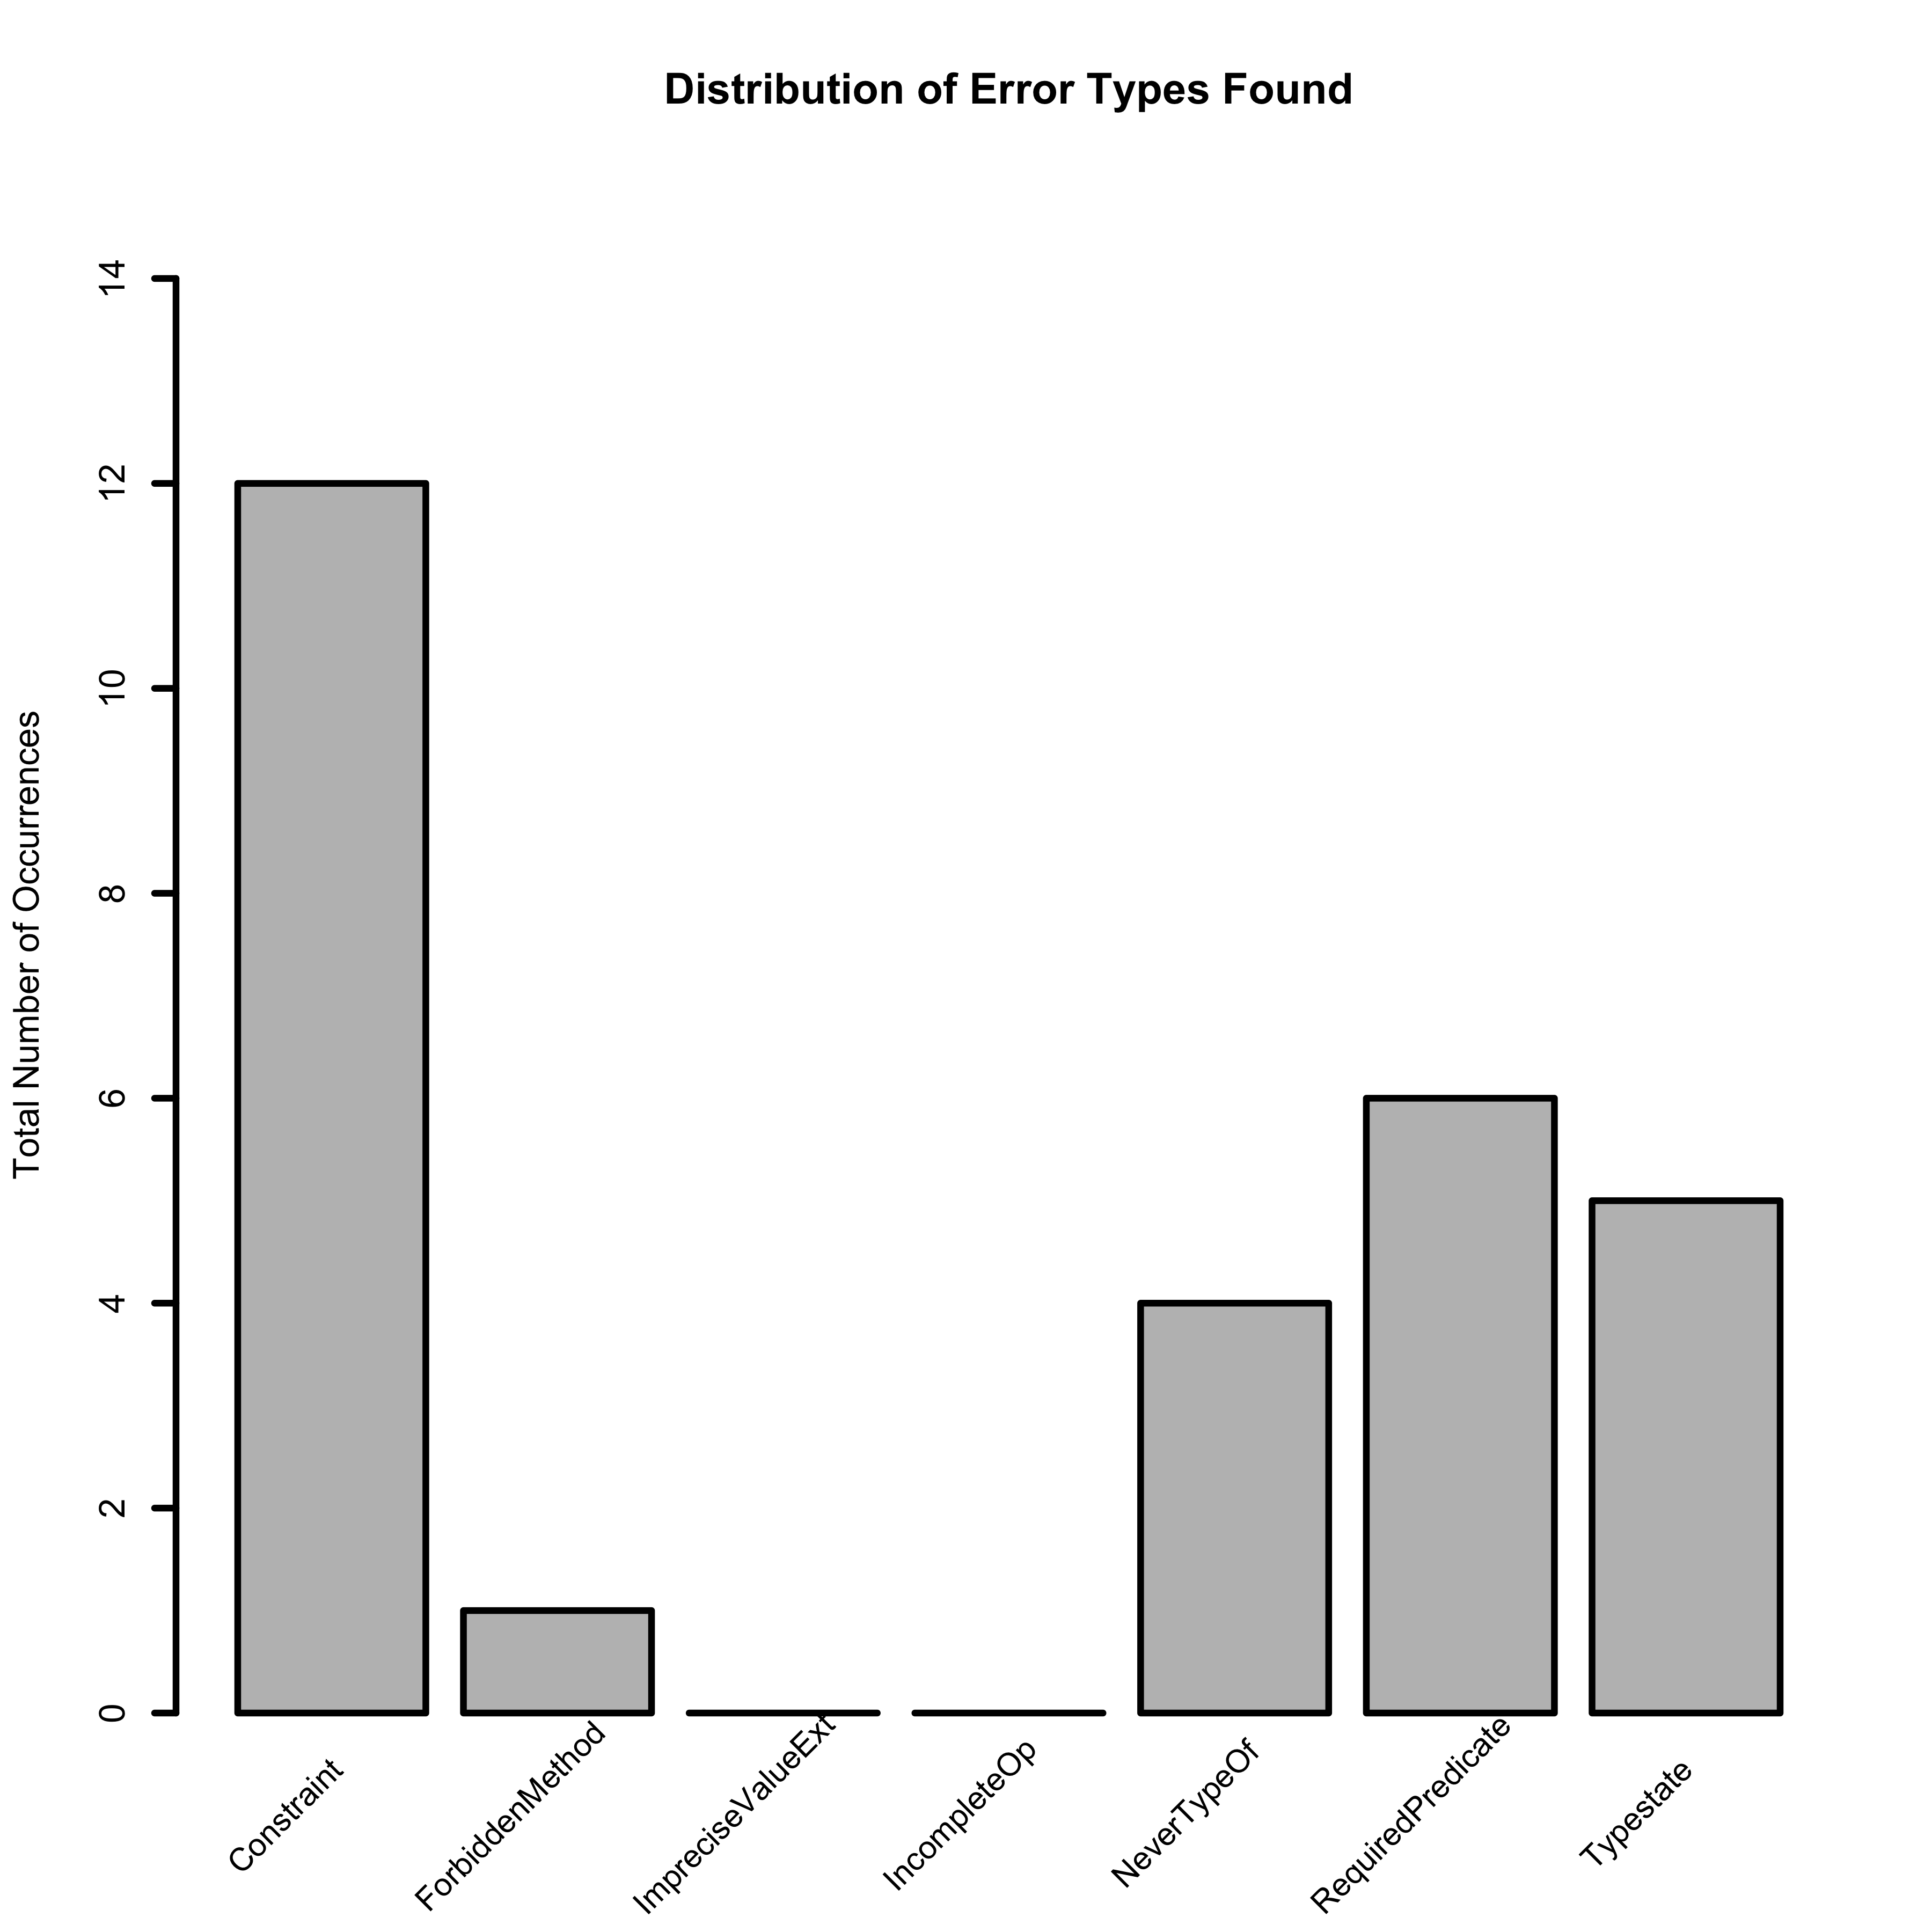
\includegraphics[width=.9\linewidth]{Dist.png}
\caption{Error types generated by CogniCrypt}
\end{center}
\end{figure}

\section{Discussion}

In light of the results that we have observed it is important to reconsider the big picture. In order to do this first we present an overview to the reader of the types of errors that CogniCrypt reports, so that we may discuss the implications of these findings.

\section{Threats to Validity}

\subsection{External Validity}
As well, we may suffer some threats to external validity due to sample size.  following ways:

\begin{itemize}
\item
It is possible that while extracting our dataset, we may miss some crypto security related posts, for example if they were not actually labelled with the java or security tag but still contain a usage of the JCA. 


\end{itemize}

\subsection{Discriminant Construct Validity}



\section{Future Improvements}
 

\section{Conclusion}

In conclusion we were able to analyze 

%\nocite{*}%not sure if you are needed.
\printbibliography

\end{document}
